\documentclass[12pt]{article}

\usepackage{rotating}		% Use sidewaystable command
\usepackage{pdflscape}		% Produce landscape pages in a (mainly) portrait document
\usepackage{float}			% Added this package to place things right where I want them!
\usepackage{mathtools}		% Added this package in order to use shortintertext command
\usepackage{amsmath}
\usepackage{amssymb}
\usepackage{geometry}
\usepackage{graphicx}
\usepackage{tikz}
\usepackage{epstopdf}
\usepackage{caption}
\usepackage{subcaption}
\usepackage{hyperref}
\usepackage[author={Harish}]{pdfcomment}

\geometry{letterpaper,tmargin=1in,bmargin=1in,lmargin=1in,rmargin=1in}
\hypersetup{
colorlinks,linkcolor=black,citecolor=violet,urlcolor=blue
}

\allowdisplaybreaks			% Allows equations to be split across multiple pages

\begin{document}

\title{System Level Design Report}
\author{Smart Vibes}
\date{December 16, 2016}
\maketitle

\newpage
\tableofcontents

\newpage
\section{Introduction}
\subsection{Product Opportunity}
Construction companies use vibrations sensors at or near construction sites of projects; they do this in order to be aware of the ground vibrations they are introducing into the surrounding area. Depending on the material composition of the buildings in the vicinity, the construction company will have a threshold value for vibration magnitudes  that they will need to stay under. Without any monitoring system, workers operating heavy machinery can cause damage to the structural integrity of the surrounding buildings. Therefore, companies like Smart Structures are in need of a system that alerts them if a construction activity or natural phenomenon has compromised the integrity of an ongoing or finished project.

\subsection{Customer Needs}
The final product will adhere to the specifications provided by Smart Structures, both in design and engineering. The new sensor will need to be portable and easy to transport, in contrast to the current ones, which are embedded into the ground. Because of this, the old sensors require any data to be recorded on site, which is costly and time consuming. Changes will not only make the new sensor solution mobile, but will also provide daily transmissions to the cloud and real time alerts. The battery included within the sensor will last up to four weeks, additionally cutting down on human interference. Also, considering the sensor will be exposed out in the construction site, it will also need to meet certain conditions such as; high and low temperature tolerance, waterproofing, and shock/impact resistance.

\subsection{Technical Specifications}
\begin{itemize}
	\item Accelerometer and geophone
	\item Monitor minimum frequency of 8Hz
	\item Local data storage
	\item Immediate emergency triggers
	\item Remote access
	\item Four week power time
	\item Cloud database
	\item Weather resistant
	\item Wifi connectivity
	\item Real-time monitoring 
	\item Server access
\end{itemize}

\subsection{Constraints}
The overall restrictions in the desired product ultimately affected its design process and implementation. While any conventional plastic case could have satisfied the housing aspect of our design, Smart Structures preferred a weatherproof enclosure. This enclosure needed to be capable of withstanding impacts and collision of high magnitudes, sub-zero temperatures, extreme heat, and moisture/precipitation. Portability was also an important factor and constraint for the case, which culminated in the current design. For prototyping; a 3-D model will be constructed in order to further assess if any changes need to be made to the composition. The finished product will ultimately be durable, yet small enough to be able to be moved to different areas, as deemed necessary.

The next design constraint that we faced was meeting the desired battery life of one month. This design required a search for low-power electronics that would keep the power usage down, but would still deliver the same performance as other power-hungry devices. For the microcontroller in the prototype, we opted to use a wifi-capable microcontroller from Adafruit. It draws very little current and can parse the data of the accelerometer and geophone sensors without a problem.

\section{System Overview}
Smart-Structures is looking for an accurate and reliable way to collect real-time ground vibrations at or around active construction sites. Construction projects are restricted in what's considered an acceptable vibration range based on the location of the project. Generally, in urban areas and near protected public places such as schools and hospitals have much lower tolerances for vibration noise.

Swiss standards SN 640 312a \cite{src1} for building damages are typically used when monitoring construction vibrations to be assured that both cosmetic and structural damage is eliminated while complaints are minimized. There are two types of fundamental mechanisms for vibration damage. The first type is distortion from inertial loads and the second is the settlement of the soils supporting the foundation. Although serious structural damage is possible, the materials that begin to crack under stress are often brittle such as drywall or plaster.

A combination of old and new techniques are used to minimize power consumption and maximize reliability. Using a strong weather-proof case, lithium polymer ion battery, geophone, accelerometer, and a microcontroller, we can accurately observe, record, and transmit valuable data. This report highlights the key features and analyzes the design, materials, electronics, potential risks, mitigation plans, and the project timeline.

\section{System Architecture}

\subsection{High Level View}
\begin{figure}[H]
    \centering
    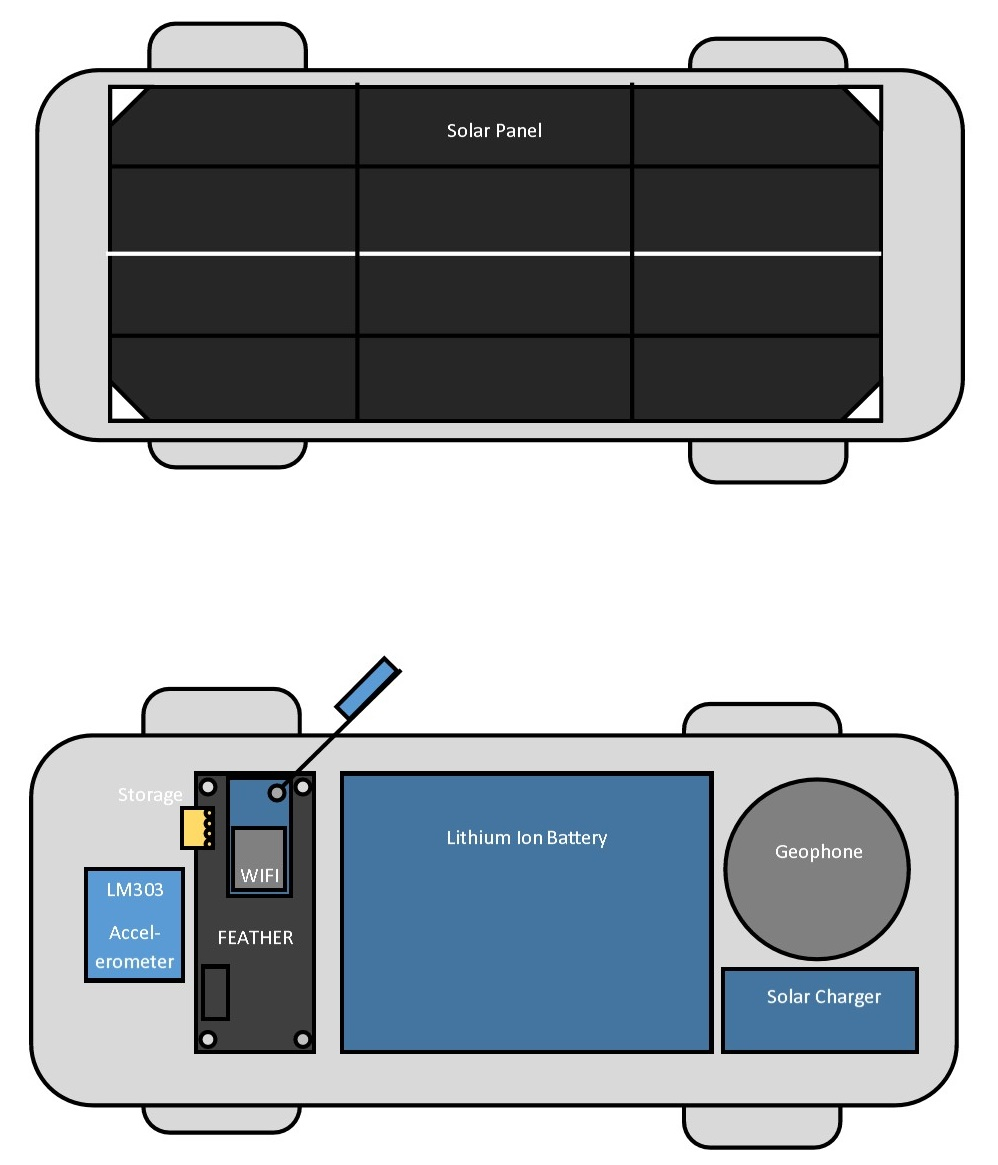
\includegraphics[width=.6\textwidth]{src/design_v2.jpg}
    \caption{Prototype design for the vibration monitoring systems. The design highlights the subsystems of the sensor. The top picture is the top view of the system. The bottom picture shows what's underneath the solar panel inside the system.}
    \label{fig:design_v2}
\end{figure}

Figure \ref{fig:design_v2} shows the prototype system designed by Smart Vibes. Data is collected from the geophone and accelerometer sensors. This data is processed by the microcontroller, for our application we are using an Adafruit Feather; a low cost, open source module that has an integrated wifi module. The chip has enough processing power to take information from the geophone and convert it to data that can be used to determine critical level vibrations. When not on alert or transmission mode, the data is stored on the SD card. The Feather has two modes, an active and a low power consumption mode, which allows for smart power usage when signals are below a threshold. At the end of day, the wifi module on the system pushes the data to the cloud where it can be viewed any time by authorized personnel at Smart Structures. The system will include an antenna, that will protrude from the case to extend the range of transmission.

\subsection{Design Rationale}
The choice for system architecture was due to three main reasons; first, the system needed to eliminate the human interaction with the collection of vibration data. Second, the system needed to be portable and withstand certain atmospheric conditions. Finally, the system had to run for at least a month before recharging.

The first issue encountered was selecting the right microcontroller. For the initial concept design a Raspberry Pi was chosen, but seeing that it would draw too much current and drain the battery quickly, it was replace with an Arduino Pro Mini microcontroller based on the Atmega processing chip. However, this would have required an extra wifi breakout board and a separate antenna board to extend the transmission range. Therefore, the final design uses an integrated microcontroller board from Adafruit that comes with a wifi module and a connection for an antenna.

The second issue with the design was finding the right battery to power the system. It was unknown what kind of battery was suitable to power all the different electronics for a full month. After, switching over from the Arduino Pro Mini to the Adafruit Feather as the microcontroller, the voltage necessary to power the entire system by analyzing the voltage requirements of all the components was finalized. All of the components in the system will run of a 3.7V battery.

Finally, the sensor housing case which had originally been designed as a flat box, was redesigned to into a dome. The dome will redistribute the force towards the edges, whereas a flat box would absorb the shock, possibly damaging the center. As far as materials go, the current preferred material is acrylonitrile butadiene styrene; also known as ABS. ABS is a common type of thermoplastic polymer that is impact resistant, durable, and heat resistant. ABS can be further strengthened by molding it at low temperatures, or adding glass fibers. This choice for housing material will ensure that the main components are safe from the elements.

\subsection{Subsystems}
Figure \ref{fig:design_v2} shows the main subsystems of the solution. The seven main subsystems in our design are the following:
\begin{itemize}
	\item Microcontroller
	\item Storage
	\item Wifi
	\item Accelerometer
	\item Geophone
	\item Battery
	\item Solar panel
\end{itemize}

\subsection{Interfaces}
For the microcontroller an Adafruit Feather was selected, which is a low-power consumption, open-source microcontroller that has an integrated wifi module. For storage requirements, an SD card attached to the Feather provides sufficient means to store data before it is pushed to the cloud database.
The Feather's integrated wifi module operates in low-power mode when it is not transmitting data.

The accelerometer senses changes in position and correlates them to ground vibrations. The geophone is composed of a spring that generates a voltage which is translated to a seismic readings. The two systems provide redundancy against erroneous readings from one sensor.

To extend the battery life of the device as much as possible, there was a need for the system to recharge the battery. Therefore, it was decided to implement and attach a solar panel to the device so that the battery can be recharged when the system is running during the day.

\subsection{Concept of Operations}
\begin{figure}[H]
    \centering
    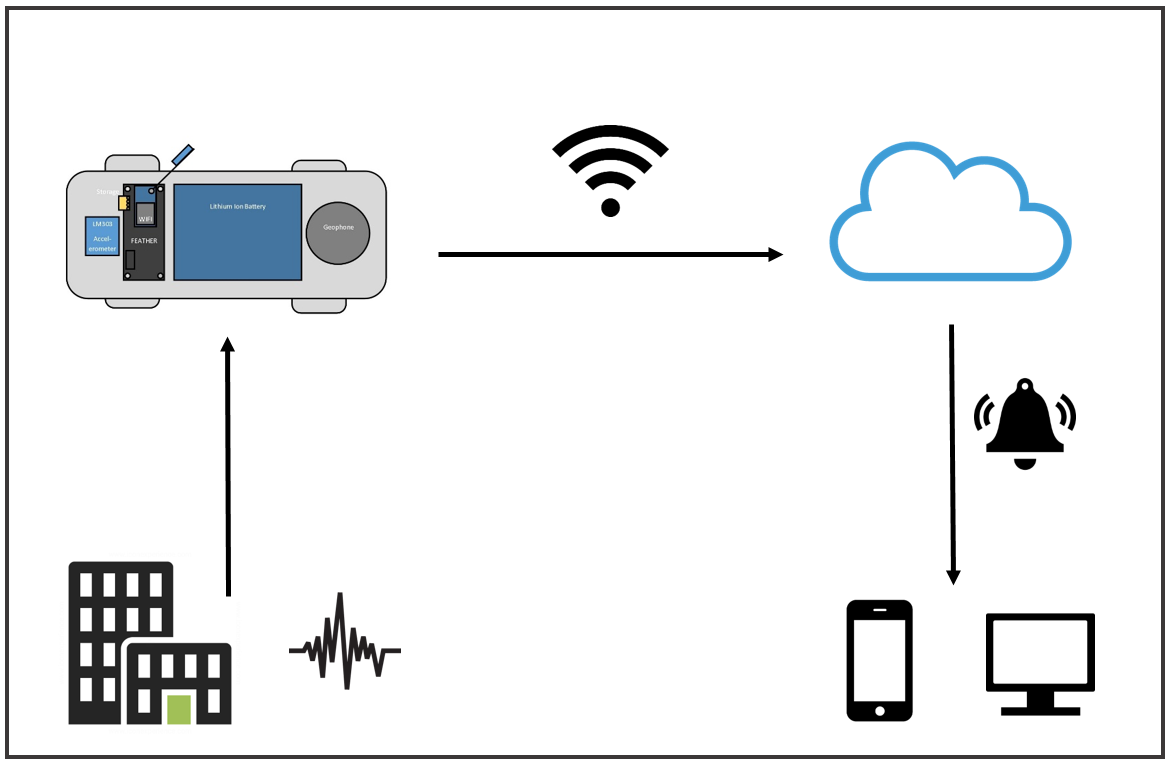
\includegraphics[width=.7\textwidth]{src/concept_of_operations.png}
    \caption{Diagram depicting the concept of operations of the vibration monitoring system.}
    \label{fig:concept_of_operations}
\end{figure}

The sensor will detect vibrations in a surrounding zone, such as construction site. It will determine one of two things; whether the vibrations are with a certain threshold or not. If not then it will send an alert via the web to someone who can respond to it. Meanwhile, it is also  constantly sampling and storing data. Once a day this data gets sent to a cloud database for analysis. Figure \ref{fig:concept_of_operations} illustrates the concept of operations with a visual.

\newpage
\section{Bill of Materials}
The bill of materials in Table \ref{tab:bom} contains tentative ``off-the-shelf'' parts that will need to be purchased in order to construct a functional prototype. The materials listed below have been selected after hours of research and fit the criteria needed to construct a weatherproofed, reliable system.
\begin{table}[H]
	\centering
	\resizebox{\columnwidth}{!}{%
	\begin{tabular}{l|l|c|l|l|l|l|c}
    	Vendor ID & Part Number & Quantity & Price/Unit & Part Description & Related Customer Need & Total Cost & Vendor \\ \hline
    	1120 & LSM303 & 2 & \$14.95 & Accelerometer & Measuring vibrations generated & \$29.90 & \href{https://www.adafruit.com/products/1120}{Adafruit} \\
    	& & & & & near a construction site. & & \\
    	2693 & N.A. & 2 & \$19.95 & 16GB MicroSD Card & Storing entire day's worth of data & \$39.90 & \href{https://www.adafruit.com/products/2693}{Adafruit} \\
    	& & & & & before it is sent to the cloud. & & \\
    	2922 & N.A. & 2 & \$8.95 & SD Card Add-On & Used to assist on-board storage & \$17.90 & \href{https://www.adafruit.com/products/2922}{Adafruit} \\
    	& & & & & of data. & & \\
    	380 & CR1220 & 2 & \$0.95 & Coin Cell Battery & Assist in the storage of data. & \$1.90 & \href{https://www.adafruit.com/products/380}{Adafruit} \\
    	3061 & N.A. & 2 & \$29.95 & Adafruit Feather & Processing and monitoring the & \$69.90 & \href{https://www.adafruit.com/products/3061}{Adafruit} \\
    	& & & & Microcontroller with Wifi & recorded vibrations. & & \\
    	353 & N.A. & 2 & \$29.50 & 6600 mAh 3.7V Lithium- & Power sensor for extended periods & \$59.00 & \href{https://www.adafruit.com/product/353}{Adafruit} \\
    	& & & & Ion Battery & of time, without needing human & & \\
    	& & & & & interaction. & & \\
    	2747 & N.A. & 1 & \$88.95 & Solar Panel & Extend the life of the battery. & \$88.95 & \href{https://www.adafruit.com/products/2747}{Adafruit} \\
    	390 & N.A. & 1 & \$17.50 & Solar Panel Adapter & Protect the battery and the & \$17.50 & \href{https://www.adafruit.com/products/390}{Adafruit} \\
    	& & & & & microcontroller. & & \\
		N.A. & 474-SEN-11744 & 1 & \$61.25 & Geophone & Measure ground vibrations. & \$61.25 & \href{http://www.mouser.com/ProductDetail/SparkFun-Electronics/SEN-11744/?qs=\%2fha2pyFaduhLW6YoPw5UUIdTRP1X\%252btPruyfOHvl8\%2fY0\%3d}{Mouser} \\
    	N.A. & N.A. & 2 & \$0.00 & Enclosure Material & House the system prototype. & \$0.00 & \href{}{3D-Printed} \\ \hline
    	Total & & & & & & \$386.20
	\end{tabular}%
	}
    \caption{Bill of materials.}
    \label{tab:bom}
\end{table}
%\begin{figure}[H]
%    \centering
%    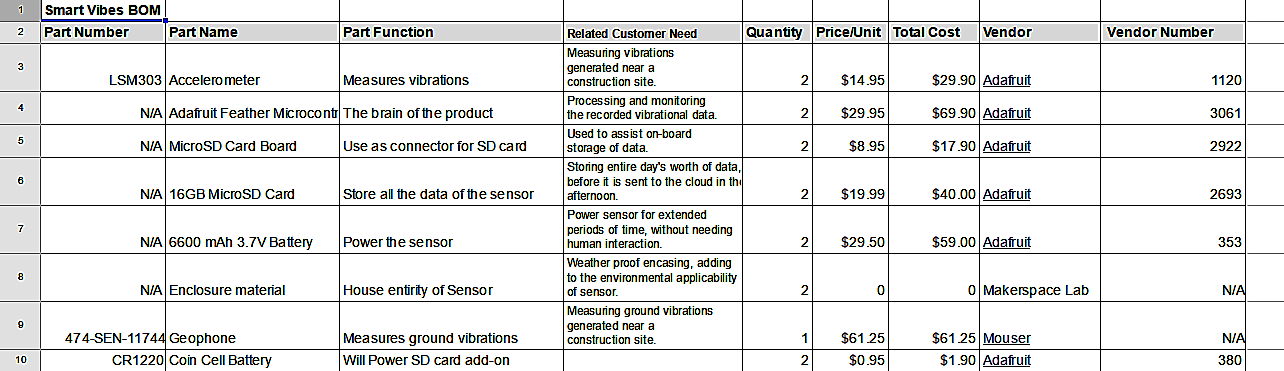
\includegraphics[width=.9\textwidth]{src/bom.png}
%    \caption{Bill of materials.}
%    \label{fig:bom}
%\end{figure}

\section{Risks}
\begin{enumerate}
\item \textbf{Case Breakage}\vspace{1mm}

\noindent The housing for the sensor must be resistant to weather, shock, dust, and other material foreign to the sensor. In the event that the exterior of the housing was not properly constructed, any impact would damage the inside components. If the housing were to break, it could introduce foreign material into the device, leading to a system failure. Therefore, the components will be covered in a waterproof case which will serve as a safeguard. The design of the case itself will be a shock proof, dome-like design which will provide a larger area for impact absorption.\\

\item \noindent \textbf{Battery Life}\vspace{1mm}

\noindent The battery needs to be able to last for the duration of peak construction periods, or up to four weeks. Due to the possibility that the device will be left outdoors for an extended duration of time, the battery needs to be able to withstand temperatures ranging from -20 to 50 degrees Celsius. This temperature range is determined from the operation range data provided in the datasheet of the battery. If this battery cannot withstand the conditions, it could ignite or leak. Another possibility is that the chosen battery will not last the required amount of time. However, the selected battery has specifications that will perform as needed under those conditions.\\

\item \noindent \textbf{Poor Surface Contact}\vspace{1mm}

\noindent If the sensor is not placed in direct contact with the surface it is measuring, there is a chance the signal will be dampened or not recorded. Loss of sensory abilities could result in a failure to detect unsafe levels of vibration. Several low and high fidelity tests will be completed to establish the limits of detection under different circumstances. With that information, an appropriate sensor design will be completed, which will have limited dampening possibilities.\\

\item \noindent \textbf{Miscalibration/Poor readings}\vspace{1mm}

\noindent Incorrect measurements could happen due to equipment malfunction or miscalibration. A minimum calibration requirement will need to be established in order to reduce any false readings. This faulty data could either miss dangerous vibrations or send an alert when there is no threat present; which could unnecessarily halt construction. To reduce the chance of that happening, rigorous calibrations will be made. \\

\item \noindent \textbf{Internet Connectivity}\vspace{1mm}

\noindent If the connectivity should fail, alerts would not be sent and important data would not be saved. The loss of connection could be due to a malfunctioning inner component, or the hotspot itself. If connectivity issues were to present themselves, the built in switch would notify the necessary personnel. This would be accomplished by programming an immediate alert to be sent if transmission is lost. 
\end{enumerate}

\subsection{Probability-Impact Matrix}
The probability-impact matrix is often used for risk management and the implementation of a mitigation plan. As seen in Figure \ref{fig:likelihood_vs_impact}, a matrix is used to plot potential risks to determine what aspect of the product or process is most vulnerable. After determining the likelihood of a problem arising, the impact of the problem is plotted. The more likely and the higher the impact the higher the risk. These high risks call for a mitigation or contingency plan to offset the possibility of a problem going wrong.
\begin{figure}[H]
    \centering
    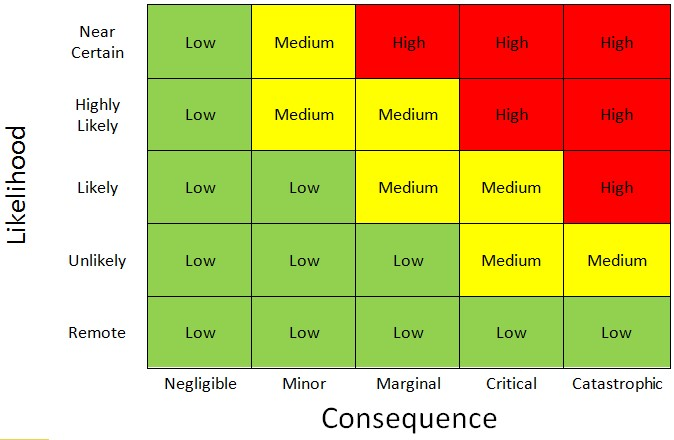
\includegraphics[width=.6\textwidth]{src/likelihood_vs_impact.png}
    \caption{Traditional probability-impact matrix. Green areas represent low risk, yellow medium risk, and red high risk.}
    \label{fig:likelihood_vs_impact}
\end{figure}

To assess the risks listed above, they were each given a number and plotted on a probability-impact matrix (Figure \ref{fig:ranked_risks}). The important thing to note is that there are overall more risks in green. The fact that there is no red-risks shows us that our design may prove to be reliable and useful. There are two risks that need to be monitored more closely, risks 1 and 4. Although unlikely breaking the case would render it useless; with its sensitive measuring equipment and electronics exposed to the elements it would not last long. Risk 4 should never occur, although, it is possible for something to go wrong during the production process or something to be missed during quality control. If the sensor does not perform as it should and sends incorrect data then construction workers may create vibrations that exceed the accepted. With incorrect data being sent it is possible to generate thousands of dollars in damage without realizing it. Our next step in this process is risk mitigation.
\begin{figure}[H]
    \centering
    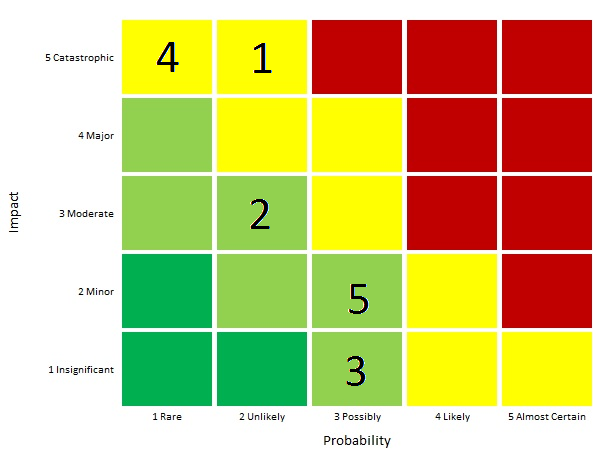
\includegraphics[width=.6\textwidth]{src/ranked_risks.png}
    \caption{The risk’s probability - impact matrix above shows the 5 ranked risks according to their likelihood and potential impact..}
    \label{fig:ranked_risks}
\end{figure}

\section{Technology Readiness Level}
Critical Design Elements - before readiness levels can be assigned, critical design elements need to be evaluated. Each of the elements below determine how well the product performs and each is a work in progress.
\begin{enumerate}
	\item Battery
	\begin{itemize}
		\item Currently the ``off-the-shelf'' battery pack being used should have enough power to reach the set requirement of 1 month.
		\item The product will evolve after much testing into a product that consumes less power and in turn lasts longer.
		\item The battery will store the energy collected from the solar panel.
	\end{itemize}
	\item Case
	\begin{itemize}
		\item The outer case of the product is planned to be made with a durable shockproof ABS plastic.
		\item Though the prototype housing will be 3D-printed, the final design next semester will incorporate ABS as the housing material. More research needs to be done next semester with ABS material.
	\end{itemize}
	\item Sensor
	\begin{itemize}
		\item Research into the vibration sensor and geophone used in the vibration monitoring system has been completed. Next semester numerous performance and calibration tests will be performed on the sensors to test durability and accuracy.
	\end{itemize}
\end{enumerate}
\begin{figure}[H]
    \centering
    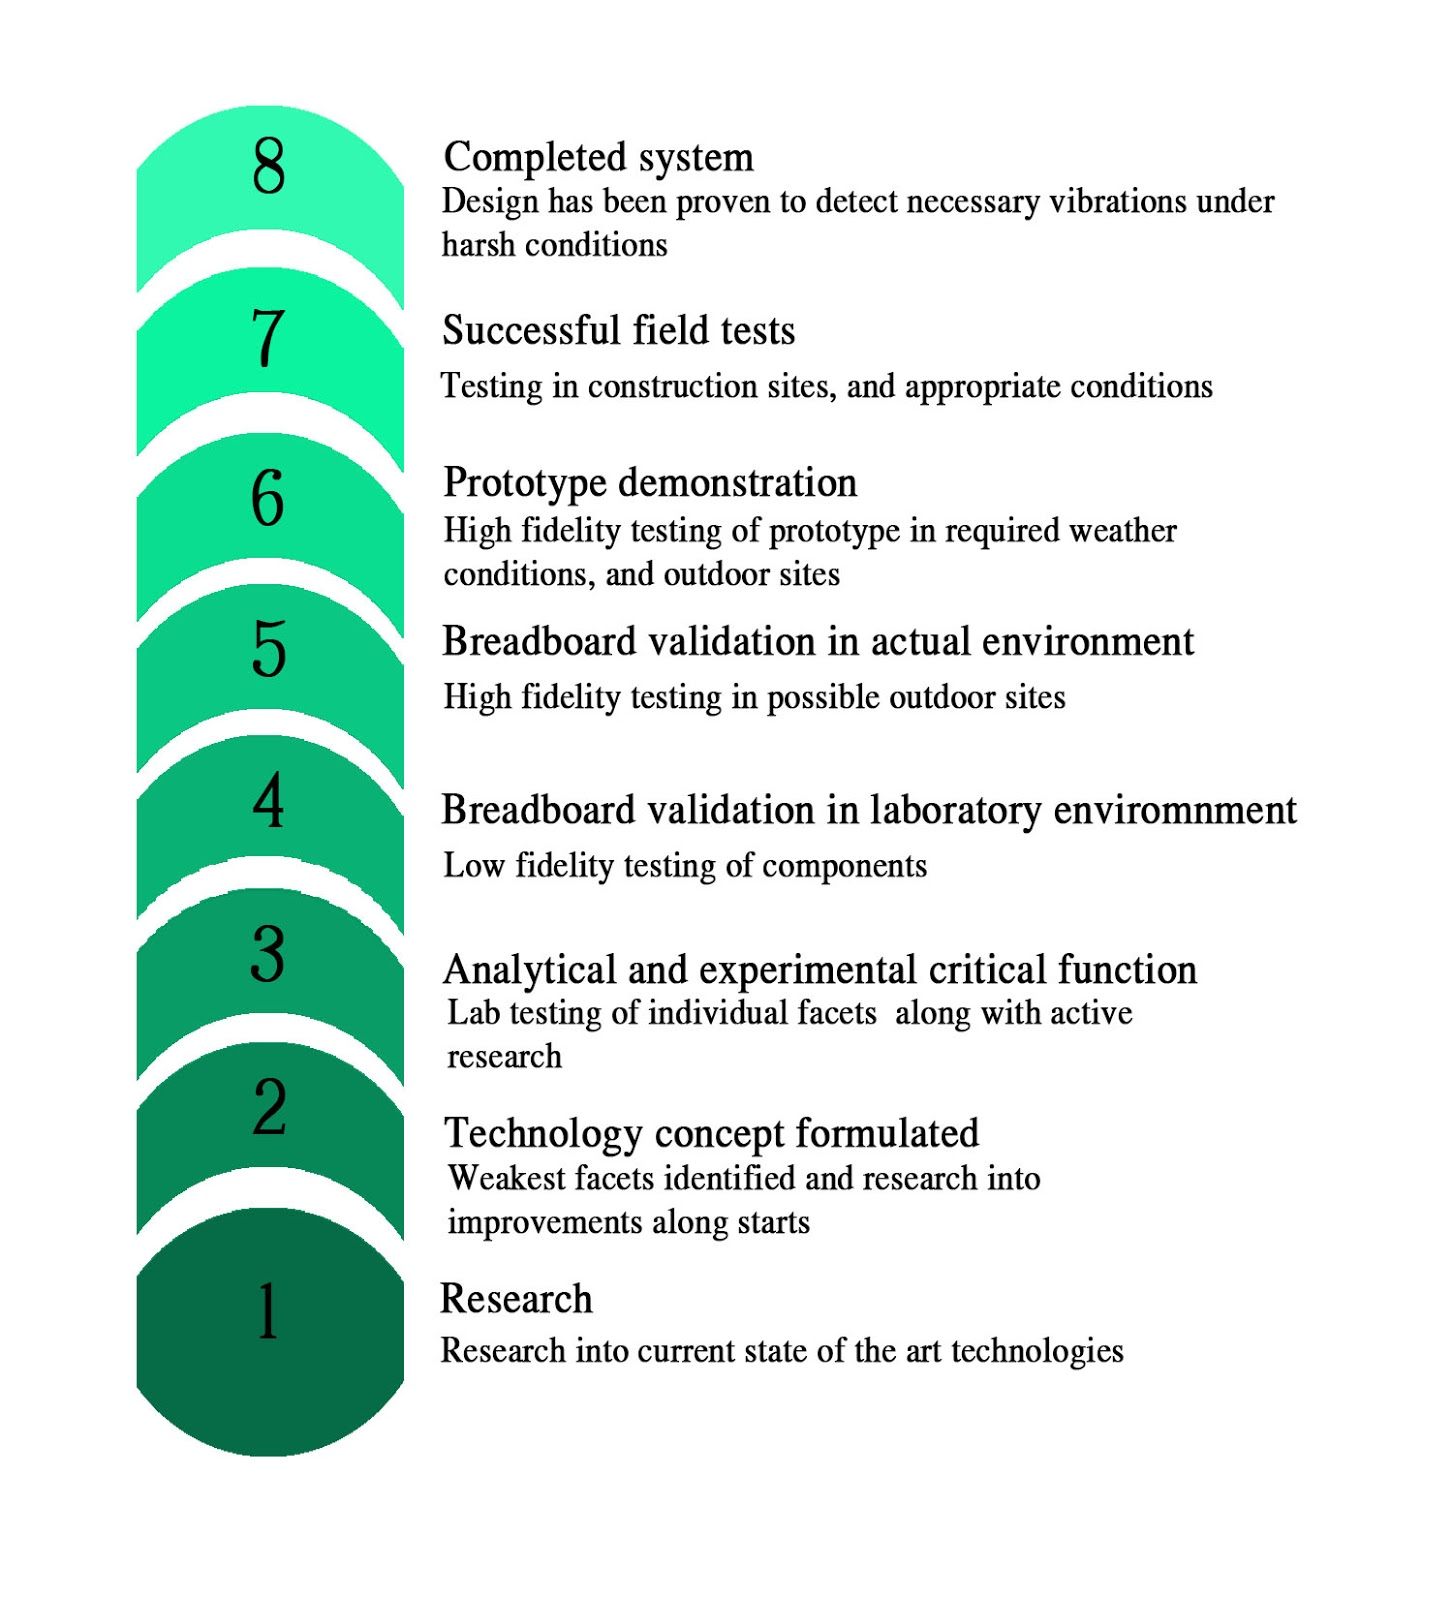
\includegraphics[width=.7\textwidth]{src/tr_level.png}
    \caption{Technology readiness levels. A generalized readiness chart depicts the stages during a project's development. Ranging from 1 through 8 it characterizes the point in product development.}
    \label{fig:tr_level}
\end{figure}

Overall our current project stands at a comfortable technology readiness level (TRL) of 3. Smart Vibes is examining individual components of the product and testing them to ensure they all work in unison. Once all this testing is done, leading up to next semester, we will begin the construction and testing in an outdoor environment. At the end of the Spring semester we will be at a TRL of 5 to 6. We will also have an operating prototype that will act as our first baseline.

\newpage
\section{Gantt Chart}
\begin{figure}[H]
    \centering
    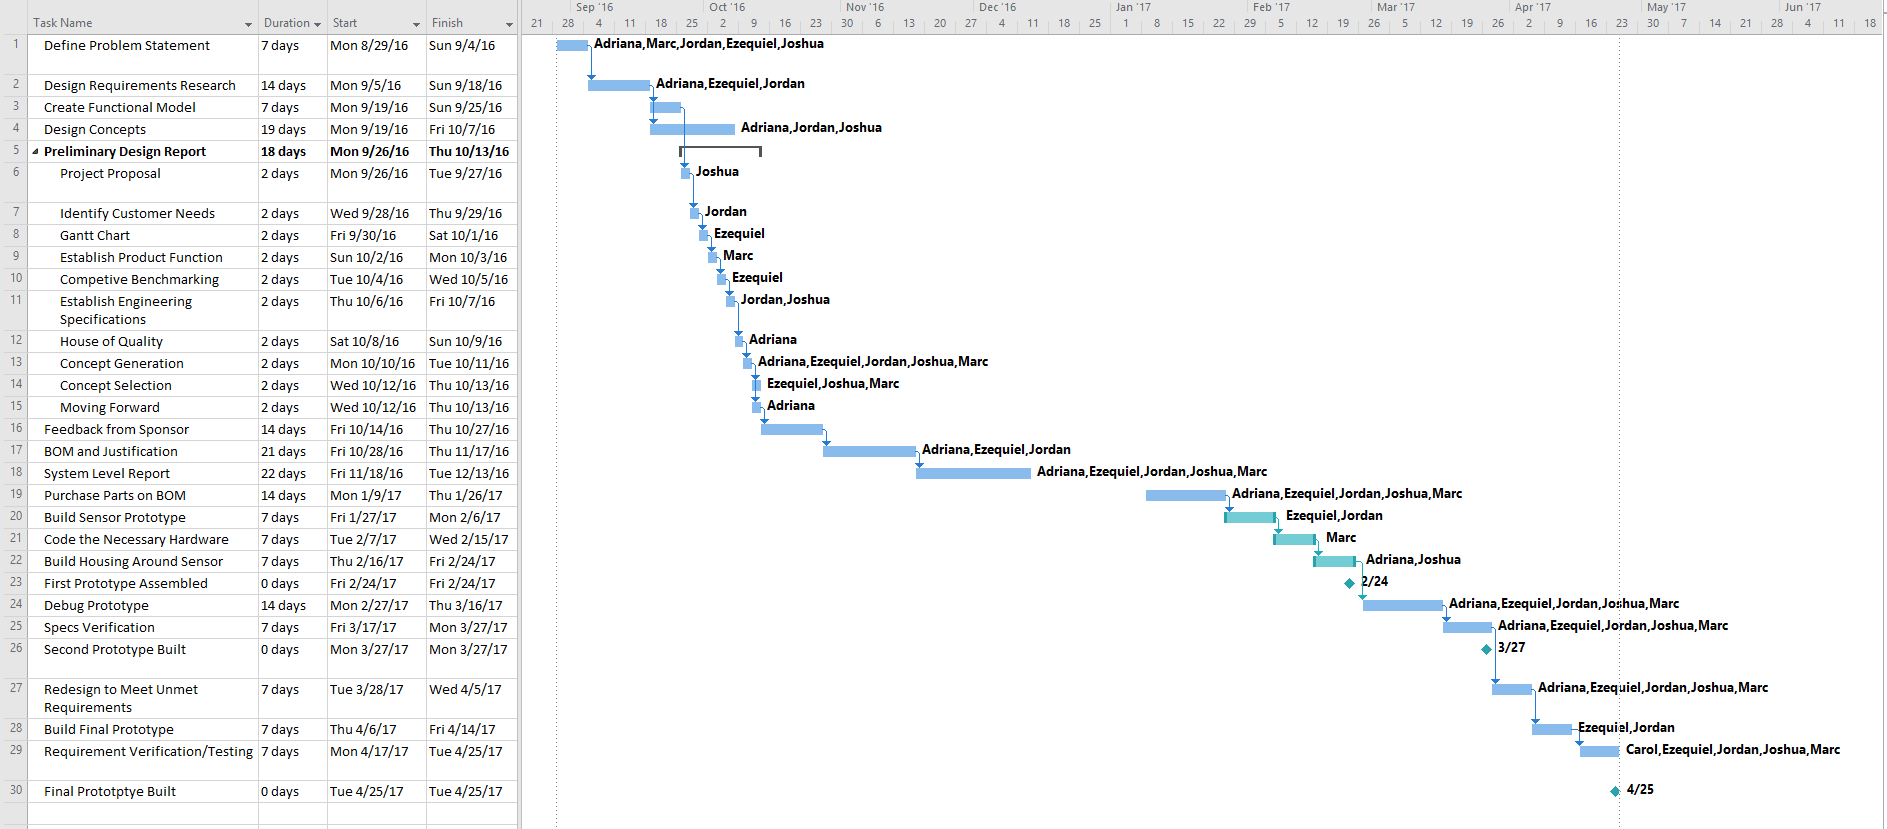
\includegraphics[width=\textwidth, angle=90]{src/gantt_chart.png}
    \caption{Project schedule. The second semester shows a couple of milestones that Smart Vibes will achieve.}
    \label{fig:gantt_chart}
\end{figure}

\newpage
\begin{thebibliography}{9}
\bibitem{src1}
``Vibration Standards.'' \textit{Vibration Standards.} N.p., n.d. Web. 17 Nov. 2016.
\bibitem{src2}
``Mining and Blasting.'' \textit{Mining and Blasting.} N.p., n.d. Web. 17 Nov. 2016.
\end{thebibliography}

\end{document}